% Ubah judul dan label berikut sesuai dengan yang diinginkan.
\section{Methodology}
\label{sec:metodologi}

% Ubah paragraf-paragraf pada bagian ini sesuai dengan yang diinginkan.


This research is conducted in accordance with the following system design along with its implementation. The system design is the concept of creating and designing infrastructure, which is then manifested in the form of flow blocks that need to be executed.

In this research, a device integrated with computer vision technology will be developed to control the movement of a wheelchair. Generally, this study will employ a system design as depicted in Figure \ref{fig:Metodologi Penelitian}.

% Gambar 3.1
\begin{figure} [ht] \centering
    % Nama dari file gambar yang diinputkan
    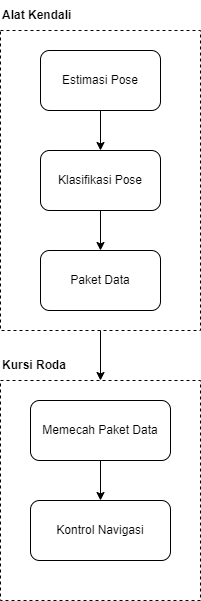
\includegraphics[scale=0.68]{gambar/blokDiagram.png}
    % Keterangan gambar yang diinputkan
    \caption{Research Block Diagram}
    % Label referensi dari gambar yang diinputkan
    \label{fig:Metodologi Penelitian}
\end{figure}

\subsection{Pose Estimation}
Pose detection is a process that involves the use of the Python programming language along with the OpenCV library and the Mediapipe framework. In this context, Mediapipe plays a crucial role in obtaining information about significant landmark points on the identified object. These landmarks then serve as the basis for creating a visual representation that visualizes the pose. The subsequent process involves connecting the specified landmark points, where lines are drawn to illustrate the spatial relationships between these points. Thus, this procedure relies not only on Mediapipe as the main framework but also utilizes OpenCV as a tool for image analysis and the visual manipulation required in pose detection.

In this study, we will leverage Mediapipe's hand pose technology to control the wheelchair's movement. Several key points, referred to as keypoints, will be utilized in this pose estimation. The keypoints selected for this pose estimation are outlined in Table \ref{tbl:titik keypoints}.

\begin{table}[h]
  \caption{Table of Relevant Keypoints for Pose Estimation\cite{Developer_2023}}
  \label{tbl:titik keypoints}
  \centering
  \begin{tabular}{|c|c|}
    \hline
    Keypoint Number& Keypoint Name     \\ \hline
    0              & Wrist              \\ \hline
    1              & Thumb CMC        \\ \hline
    2              & Thumb MPM        \\ \hline
    3              & Thumb IP         \\ \hline
    4              & Thumb TIP        \\ \hline
    5              & Index Finger MCP       \\ \hline
    6              & Index Finger PIP       \\ \hline
    7              & Index Finger DIP       \\ \hline
    8              & Index Finger TIP       \\ \hline
    9              & Middle Finger MCP     \\ \hline
    10             & Middle Finger PIP     \\ \hline
    11             & Middle Finger DIP     \\ \hline
    12             & Middle Finger TIP     \\ \hline
    13             & Ring Finger MCP     \\ \hline
    14             & Ring Finger PIP     \\ \hline
    15             & Ring Finger DIP     \\ \hline
    16             & Ring Finger TIP     \\ \hline
    17             & Pinky Finger MCP     \\ \hline
    18             & Pinky Finger PIP     \\ \hline
    19             & Pinky Finger DIP     \\ \hline
    20             & Pinky Finger TIP     \\ \hline
  \end{tabular}
\end{table}

Each landmark point on the model will be colored with a unique color to distinguish each finger. Specifically, the color assigned to each landmark point reflects its association with a specific finger, thereby creating a more detailed and informative visual representation. To provide a more concrete illustration, the following is an example image of the estimated pose, as shown in Figure \ref{fig:contoh citra yang telah diestimasi pose}

\begin{figure} [ht] \centering
  % Nama dari file gambar yang diinputkan
  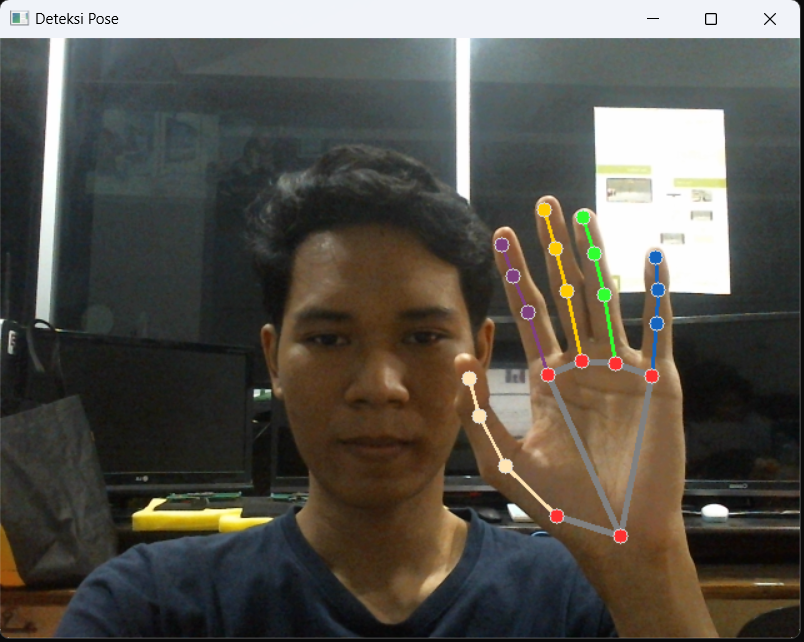
\includegraphics[scale=0.5]{gambar/bab3/EstimasiPose.png}
  % Keterangan gambar yang diinputkan
  \caption{Example image of the estimated pose}
  % Label referensi dari gambar yang diinputkan
  \label{fig:contoh citra yang telah diestimasi pose}
\end{figure}

\newpage

\subsection{Pose Classification}
After the hand pose estimation process is completed, the next step involves grouping the images resulting from the estimation into a dataset. This dataset will have 5 different classes, each representing commands for forward, backward, right movement, left movement, and stop. These classes represent the basic commands for controlling the wheelchair. 

To enhance performance and accuracy, this dataset will undergo a training process using the Convolutional Neural Network (CNN) algorithm. The utilization of CNN in training the dataset is expected to produce a model capable of recognizing complex patterns and features, allowing the system to respond appropriately to various commands that may be given by the user. The results of the generated prediction model can be observed in Figure \ref{fig:klasifikasi kiri}, Figure \ref{fig:klasifikasi maju}, Figure \ref{fig:klasifikasi stop}, Figure \ref{fig:klasifikasi mundur}, and Figure \ref{fig:klasifikasi kanan}.

\begin{figure} [h] \centering
  % Nama dari file gambar yang diinputkan
  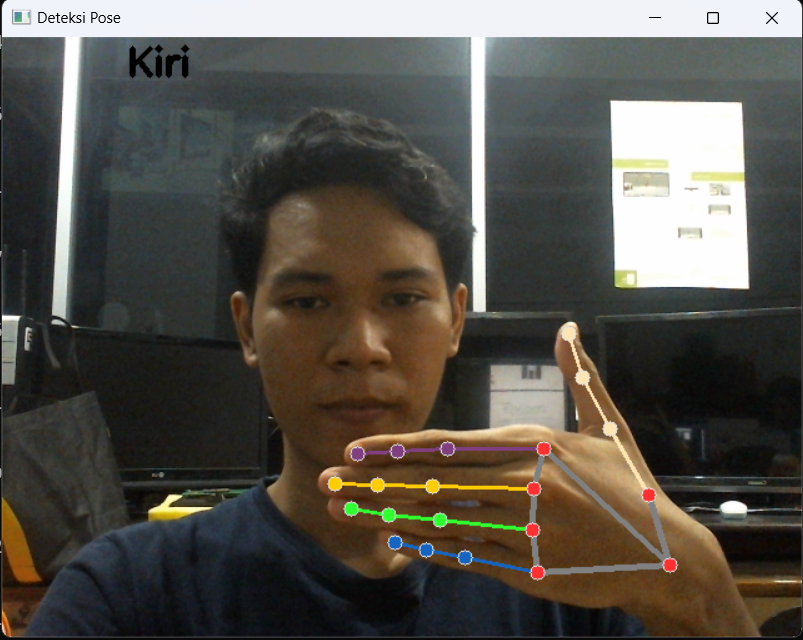
\includegraphics[scale=0.48]{gambar/bab3/Kiri.png}
  % Keterangan gambar yang diinputkan
  \caption{Example image detecting left}
  % Label referensi dari gambar yang diinputkan
  \label{fig:klasifikasi kiri}
\end{figure}

\begin{figure} [h] \centering
  % Nama dari file gambar yang diinputkan
  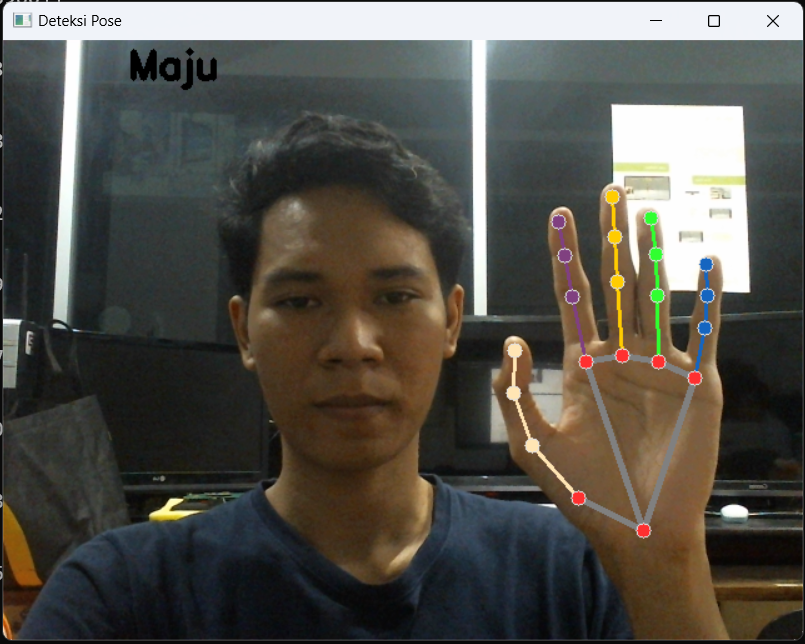
\includegraphics[scale=0.48]{gambar/bab3/Maju.png}
  % Keterangan gambar yang diinputkan
  \caption{Example image detecting forward}
  % Label referensi dari gambar yang diinputkan
  \label{fig:klasifikasi maju}
\end{figure}

\begin{figure} [h] \centering
  % Nama dari file gambar yang diinputkan
  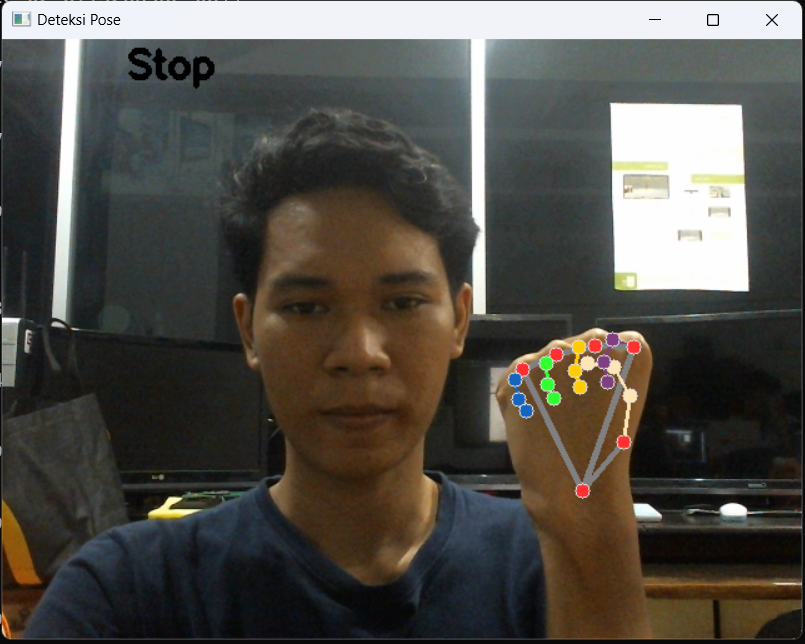
\includegraphics[scale=0.48]{gambar/bab3/Stop.png}
  % Keterangan gambar yang diinputkan
  \caption{Example image detecting a stop}
  % Label referensi dari gambar yang diinputkan
  \label{fig:klasifikasi stop}
\end{figure}

\begin{figure} [!ht] \centering
  % Nama dari file gambar yang diinputkan
  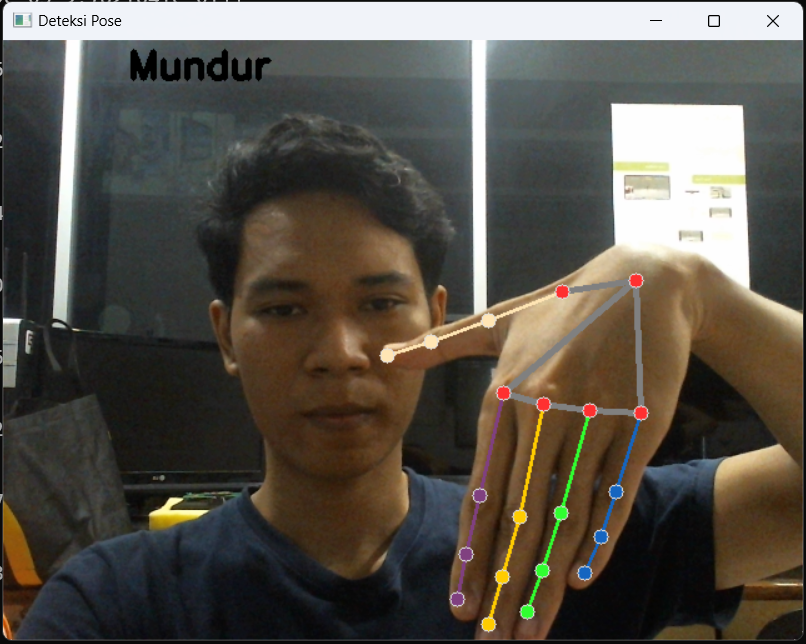
\includegraphics[scale=0.48]{gambar/bab3/Mundur.png}
  % Keterangan gambar yang diinputkan
  \caption{Example image detecting reverse or backward}
  % Label referensi dari gambar yang diinputkan
  \label{fig:klasifikasi mundur}
\end{figure}

\begin{figure} [!h] \centering
  % Nama dari file gambar yang diinputkan
  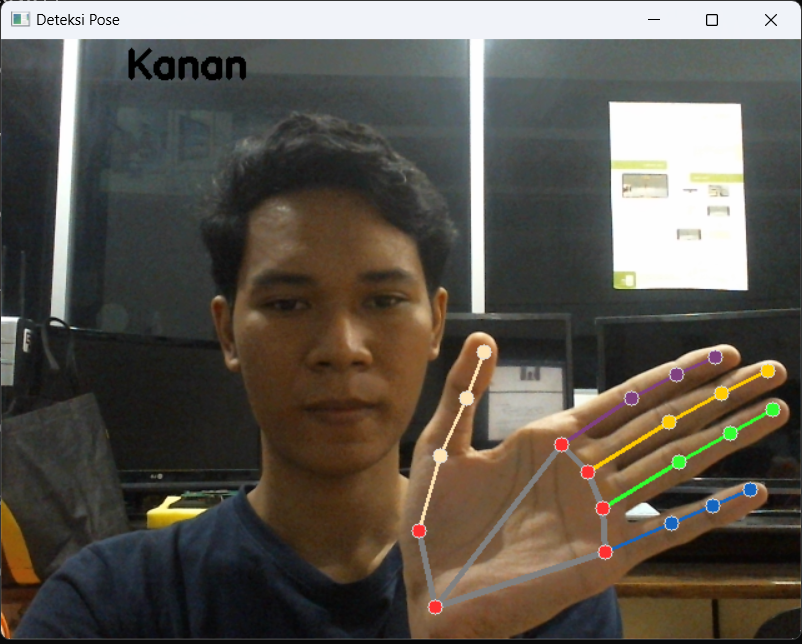
\includegraphics[scale=0.48]{gambar/bab3/Kanan}
  % Keterangan gambar yang diinputkan
  \caption{Example image detecting right}
  % Label referensi dari gambar yang diinputkan
  \label{fig:klasifikasi kanan}
\end{figure}

\newpage

\subsection{Data Package}
In order to move the wheelchair, it is necessary to send commands to the wheelchair controller. In the pose classification stage, basic commands for wheelchair movement, such as forward, backward, right, left, and stop, have been obtained. These commands will then be combined with the maximum speed to form a single command or data package, as seen in Equation \ref{eq:paket-data}.

% Persamaan 3.1
\begin{equation}
  \label{eq:paket-data}
    Direction(char),Speed(integer)
\end{equation}

The direction variable has a data type of char that will determine the movement of the wheelchair's motor, while the speed variable has an integer data type that will specify the maximum speed of the wheelchair. To minimize data size, the instruction codes for determining the direction of movement use a single letter to represent each movement. The instruction codes can be seen in Table \ref{tbl:kode-instruksi}. 

% Tabel 3.2
\begin{table}[h]
  \centering
      \caption{The instruction codes from the pose classification results}
      \label{tbl:kode-instruksi}
      \begin{tabular}{|c|c|}
          \hline
          Klasifikasi Pose & Kode Instruksi \\ \hline
          Kiri             & A              \\ \hline
          Maju             & B              \\ \hline
          Stop             & C              \\ \hline
          Mundur           & D              \\ \hline
          Kanan            & E              \\ \hline
      \end{tabular}
\end{table}

After combining both variables, they will be wirelessly transmitted, either using Bluetooth or WiFi, from a laptop or Jetson Nano to the ESP32.

\subsection{Decode Data Package}
The data package sent through the laptop or Jetson Nano will be received by the ESP32 using Bluetooth or WiFi. Upon reception by the ESP32, the data undergoes a series of processes involving data package decoding and adjustment according to the predefined variables. This decoding process allows the ESP32 to decompose the information contained in each package and ensure that each variable is accurately separated. Thus, this process organizes and rearranges the information, ensuring that each variable aligns correctly with the provided variable names and data types.

\subsection{Navigation Control}
Both variables obtained from decoding the data package will be processed on the ESP32. The direction variable will play a role in determining the motor's movement direction, while the speed variable will be used to set the maximum speed of the motor movement. There is a series of chained 'if' logics in the navigation control, where the four direction variables will determine the motor rotation direction. Additionally, the maximum PWM value is configured using the speed variable, allowing users to adjust the maximum motor speed as desired. Thus, at this stage, the ESP32 can effectively process the data received through the wireless system and generate corresponding control instructions to move the wheelchair in the desired direction and speed.